\documentclass[12pt]{article}
\usepackage{graphicx,float}
\usepackage{listings}
\usepackage{xcolor}
\usepackage{circuitikz}

\graphicspath{ {./fig/} }

\definecolor{codegreen}{rgb}{0,0.6,0}
\definecolor{codegray}{rgb}{0.5,0.5,0.5}
\definecolor{codepurple}{rgb}{0.58,0,0.82}
\definecolor{backcolour}{rgb}{0.95,0.95,0.92}


\lstdefinelanguage{SPICE}{
  keywords={tran,ac,dc,subckt,meas,plot,print,control,run,end,endc, hardcopy},
  morecomment=[l]{*},
  morecomment=[l]{\$},
  morecomment=[s]{/*}{*/},
  morestring=[b]',
  morestring=[b]",
  ndkeywords={r,r1,r2,r3,r4,r5,l,l1,l2,l3,l4,l5,c,c1,c2,c3,c4,c5,v,vin,m,m1,m2,m3,m4,m5,d,d1,d2,d3,d4,d5,vdb, pulse,sin,i,pwl,exp},
  keywordstyle=\color{blue}\bfseries,
  ndkeywordstyle=\color{codegreen}\bfseries,
  identifierstyle=\color{black},
  commentstyle=\color{purple}\ttfamily,
  stringstyle=\color{red}\ttfamily,
  sensitive=true
}
\lstdefinestyle{mystyle}{
	backgroundcolor=\color{backcolour},   
    commentstyle=\color{codegreen},
    keywordstyle=\color{magenta},
    numberstyle=\tiny\color{codegray},
    stringstyle=\color{codepurple},
    basicstyle=\ttfamily\footnotesize,
    breakatwhitespace=false,         
    breaklines=true,                 
    captionpos=b,                    
    keepspaces=true,                 
    numbers=left,                    
    numbersep=5pt,                  
    showspaces=false,                
    showstringspaces=false,
    showtabs=false,                  
    tabsize=4
}

\lstset{style=mystyle}


% Title[Enter title of the experiment here]
\title{EE230: Lab-3\\
Precision Rectifier using Opamp}

% Author[Enter details of author here]
\author{Prateek Garg, 20D070060}

% begin the document.
\begin{document}
\noindent
% make a title page.[this creates title page]
\maketitle

\section{Overview of the experiment} %[This segment creates Section as seen in document]

\subsection{Aim of the experiment}%[This segment creates sebsections under the same section]
The aim of the experiment is to create a improved design of Hal-wave and full-wave rectifiers using Opamps 
and then simulate the designs in ngspice.
\subsection{Methods}
\subsubsection{Half-wave Precision Rectifier}
We use the opamp circuit file \texttt{ua741.txt} and \texttt{Diode\_1N914.txt} file for Diode circuit. 
Using two different diode configurations we make two Half-Wave rectifier circuits working on alternate cycles of inputs 
\subsubsection{Full-wave Precision Rectifier}
We use the opamp circuit file \texttt{ua741.txt} and \texttt{Diode\_1N914.txt} file for Diode circuit. 
We start by defining subcircuits for Half-Wave rectifier and another subcircuit for Inverting-Summer. Then the netlist was used to describe connections.


All the designs were simulated on Ngspice and exporting the values to a python script to plot them using Matplotlib.
\section{Design}
\subsection{Half Wave Rectifier A}
\begin{figure}[H]
  \begin{center}
    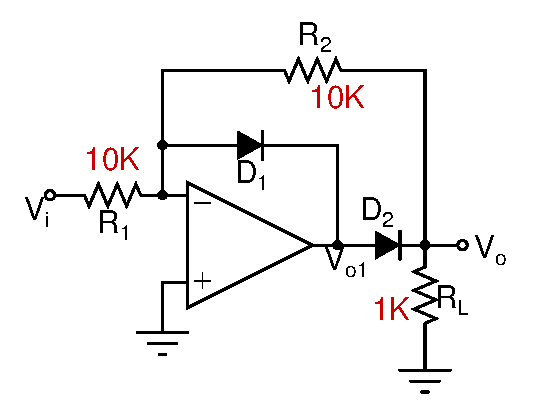
\includegraphics{hwa.eps}
\end{center}
\end{figure}
\subsection{Half Wave Rectifier B}
\begin{figure}[H]
  \begin{center}
    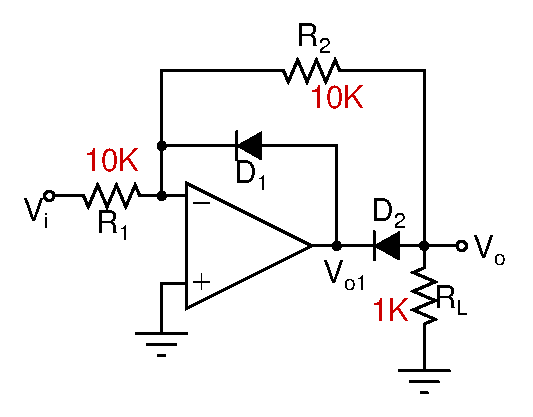
\includegraphics{hwb.eps}
\end{center}
\end{figure}
\subsection{Full Wave Rectifier}
\begin{figure}[H]
  \begin{center}
    \makebox[0.8\textwidth]{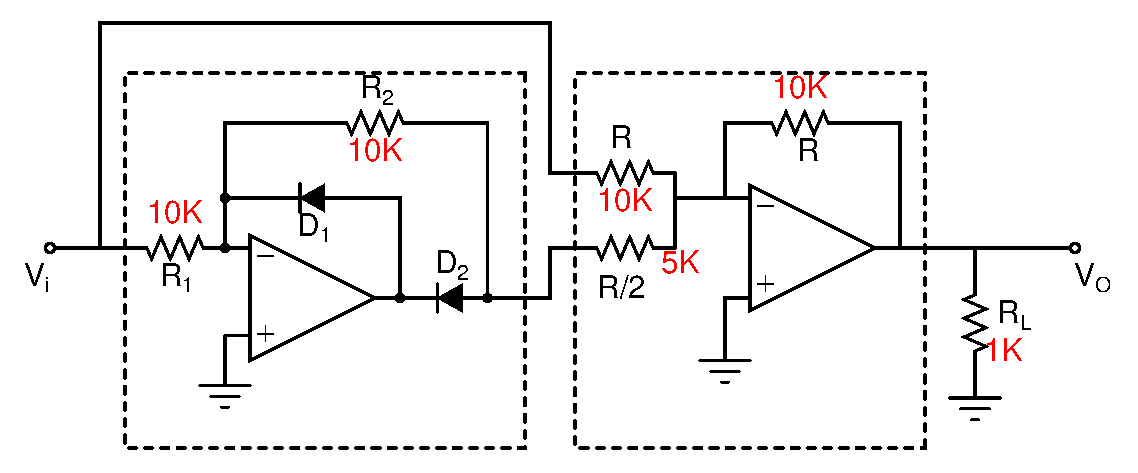
\includegraphics[width=0.8\paperwidth]{fwr.eps}}
\end{center}
\end{figure}

\section{Simulation results}

\subsection{Half Wave Rectifier A}
\subsubsection{Code snippet}
\lstinputlisting[language=SPICE]{../Improved-half-waver-rectfier-A.cir}
\subsubsection{Simulation results}
\makebox[\textwidth]{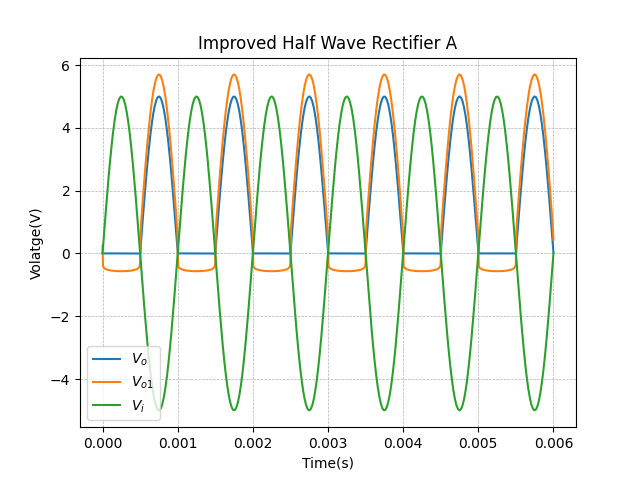
\includegraphics[width=\paperwidth]{Improved-Half-Wave-Rectifier-A.png}}

\subsection{Half Wave Rectifier B}
\subsubsection{Code snippet}
\lstinputlisting[language=SPICE]{../Improved-half-waver-rectfier-B.cir}
\subsubsection{Simulation results}
\makebox[\textwidth]{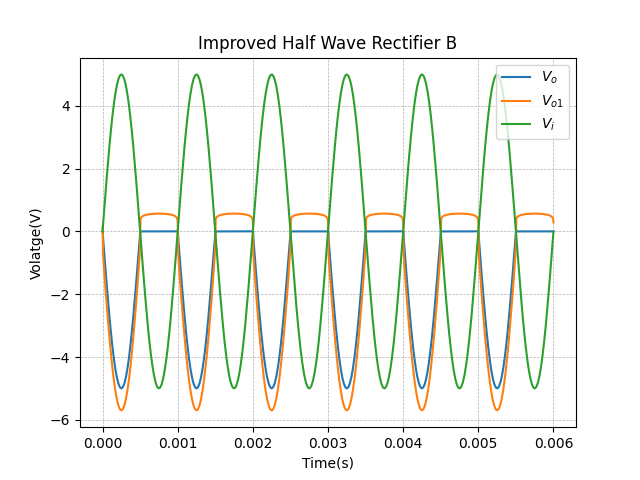
\includegraphics[width=\paperwidth]{Improved-Half-Wave-Rectifier-B.png}}

\subsection{Full Wave Rectifier}
\subsubsection{Code snippet}
\lstinputlisting[language=SPICE]{../Full-Wave-Rectifier.cir}
\subsubsection{Simulation results}
\makebox[\textwidth]{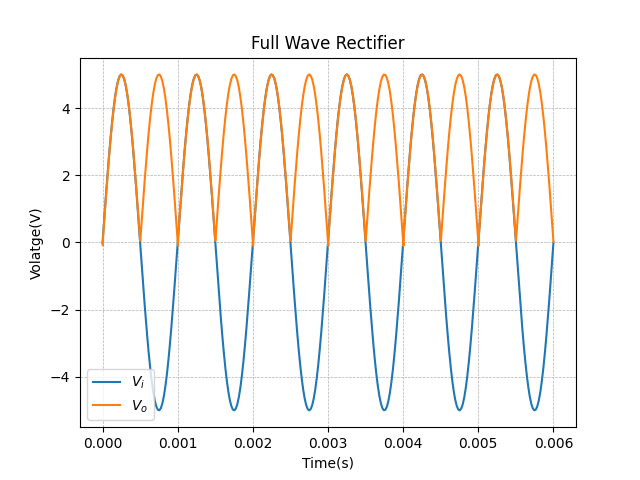
\includegraphics[width=\paperwidth]{Full-Wave-Rectifier.png}}

\section{Experimental results}
\subsection{Half Wave Rectifier A}
\begin{figure}[H]
  \begin{center}
\makebox[0.5\textwidth]{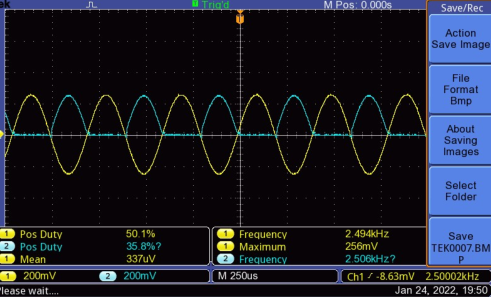
\includegraphics[width=0.5\paperwidth]{hwa-e.png}}
\end{center}
\end{figure}
The experimental results match theoretical predictions quite well.

\subsection{Half Wave Rectifier B}
\begin{figure}[H]
  \begin{center}
\makebox[0.5\textwidth]{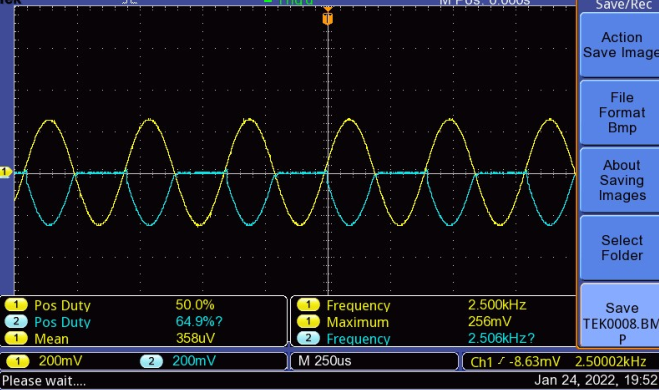
\includegraphics[width=0.5\paperwidth]{hwb-e.png}}
\end{center}
\end{figure}
The experimental results match theoretical predictions quite well. 

\subsection{Full Wave Rectifier}
\begin{figure}[H]
  \begin{center}
    \makebox[0.5\textwidth]{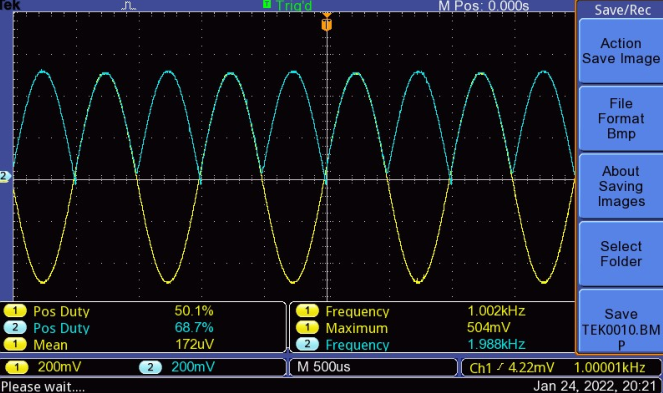
\includegraphics[width=0.5\paperwidth]{fwre.png}}  
  \end{center}
\end{figure}
The experimental results match theoretical predictions quite well.

\section{Experiment completion status}
All the sections were completed
\end{document}
